% Szglab4
% ===========================================================================
%


\chapter{Prototípus koncepciója}

A módosult diagrammok:

\begin{figure}[h]
	\begin{center}
		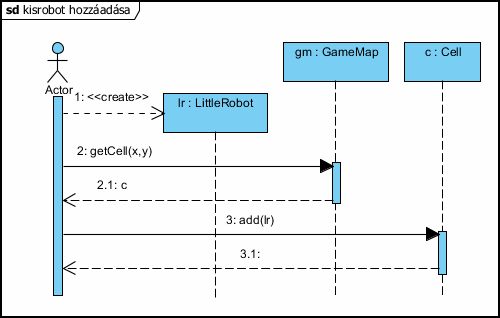
\includegraphics[width=11cm]{chapters/chapter01/kisrobot_hozzaadasa.png}
		\caption{Kisrobot hozzáadása}
		\label{fig:SzkeletonUseCase}
	\end{center}
\end{figure}


\begin{figure}[h]
	\begin{center}
		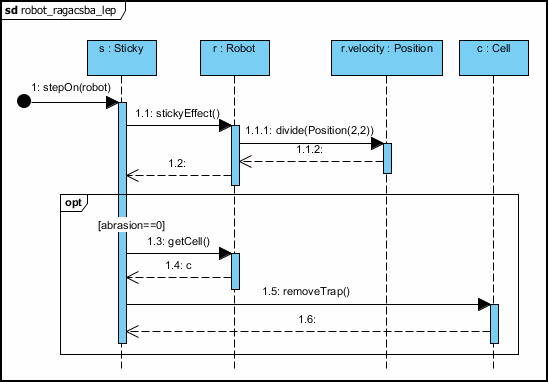
\includegraphics[width=11cm]{chapters/chapter01/robot_ragacsba_lep.png}
		\caption{Robot ragacsba lép}
		\label{fig:SzkeletonUseCase}
	\end{center}
\end{figure}

\clearpage


\begin{figure}[h]
	\begin{center}
		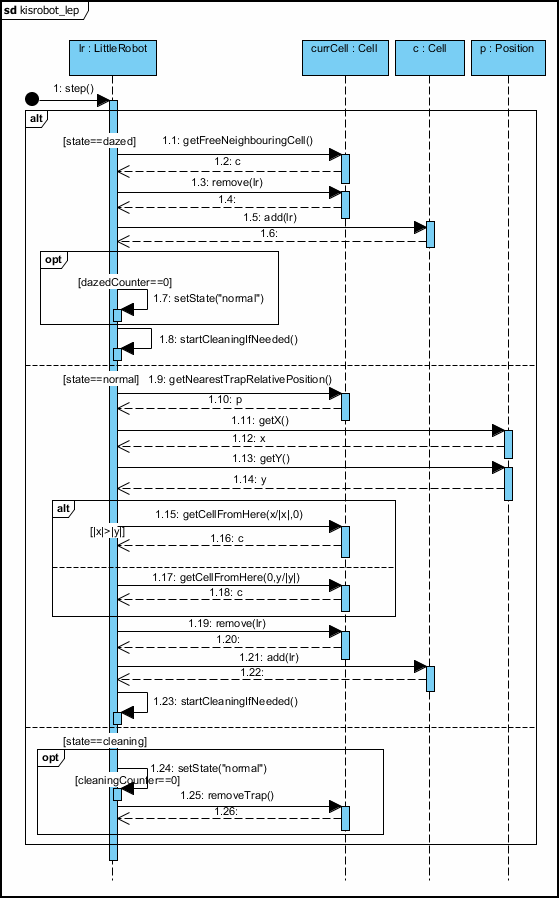
\includegraphics[width=15cm]{chapters/chapter01/kisrobot_lep.png}
		\caption{Kisrobot lép}
		\label{fig:SzkeletonUseCase}
	\end{center}
\end{figure}

\clearpage

\begin{figure}[h]
	\begin{center}
		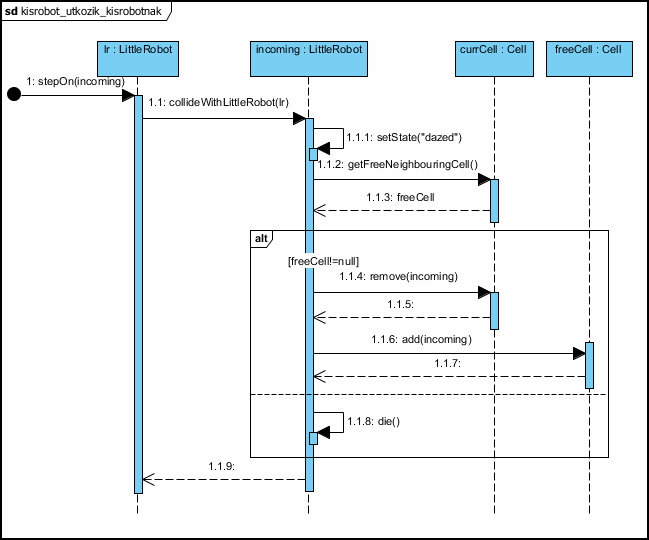
\includegraphics[width=110mm]{chapters/chapter01/kisrobot_utkozik_kisrobotnak.png}
		\caption{Kisrobot ütközik kisrobotnak}
		\label{fig:SzkeletonUseCase}
	\end{center}
\end{figure}

\begin{figure}[h]
	\begin{center}
		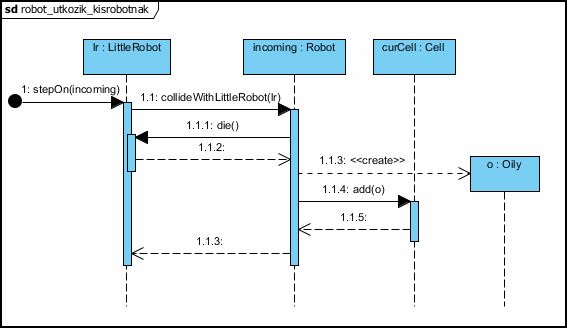
\includegraphics[width=110mm]{chapters/chapter01/robot_utkozik_kisrobotnak.png}
		\caption{Robot ütközik kisrobotnak}
		\label{fig:SzkeletonUseCase}
	\end{center}
\end{figure}
\clearpage

\begin{figure}[h]
	\begin{center}
		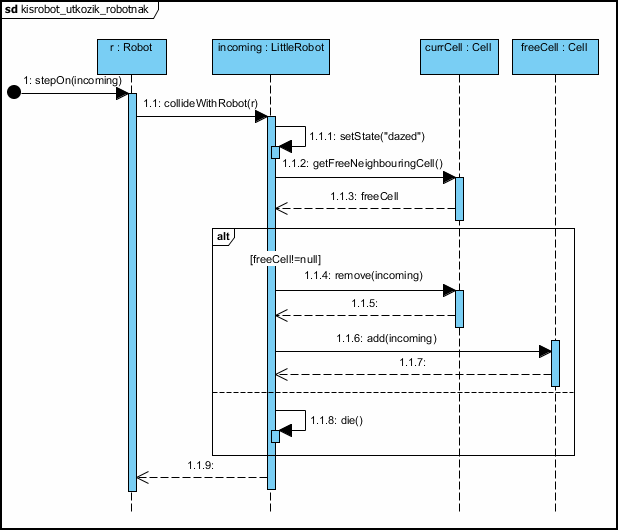
\includegraphics[width=17cm]{chapters/chapter01/kisrobot_utkozik_robotnak.png}
		\caption{Kisrobot ütközik robotnak}
		\label{fig:SzkeletonUseCase}
	\end{center}
\end{figure}
\clearpage

\begin{figure}[h]
	\begin{center}
		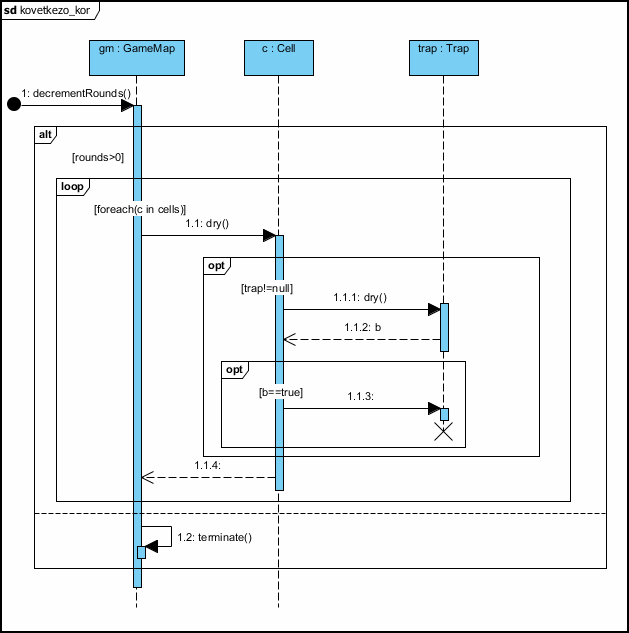
\includegraphics[width=17cm]{chapters/chapter01/kovetkezo_kor.png}
		\caption{Következő kör}
		\label{fig:SzkeletonUseCase}
	\end{center}
\end{figure}
\clearpage


\begin{figure}[h]
	\begin{center}
		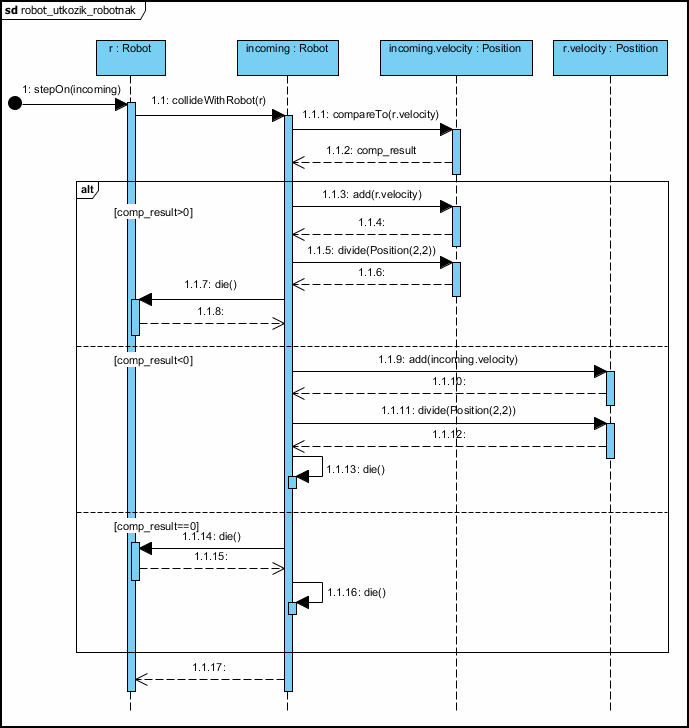
\includegraphics[width=17cm]{chapters/chapter01/robot_utkozik_robotnak.png}
		\caption{Robot ütközik robotnak}
		\label{fig:SzkeletonUseCase}
	\end{center}
\end{figure}
\clearpage
\begin{figure}[h]
	\begin{center}
		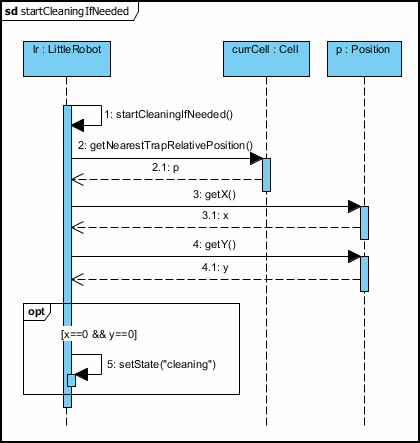
\includegraphics[width=17cm]{chapters/chapter01/startcleaningifneeded.png}
		\caption{Start cleaning if needed}
		\label{fig:SzkeletonUseCase}
	\end{center}
\end{figure}
\clearpage

\thispagestyle{fancy}

\section{Prototípus interface-definíciója}

\subsection{Az interfész általános leírása}

A program a végrehajtandó utasításokat parancsok formájában várja. Lehetőség van a parancsokat egy
szövegfájlban előre megírni. A program elindításakor argumentumok formájában kell megadni, hogy a
végrehajtandó parancsok melyik fájlban vannak tárolva (második argumentum), illetve hogy az állapotjelentés
mentése mely fájlba történjen (harmadik argumentum).
A programnak kötelező átadni még egy parancssori Argumentumot méghozzá azt hogy debug módban fut-e a program, vagy sima teszt üzemmódban. Az argumentum értékei DEBUG\_ON ÉS DEBUG\_OFF lehetnek. Debug üzemmódban az eredmény fileok hasznos event logokat tartalmaznak, amíg sima üzemmódban csak azokat az információkat, amiket parancsokkal kértünk le a teszteset kódjában.
Az Például, ha a programot a java Program DEBUG\_OFF test1.txt
eredmeny.txt formájában indítjuk, akkor ebben az esetben bemenetként a „test1.txt”, kimeneti fájlként az
„eredmeny.txt” szolgál. A pályát ugyanazzal a parancsnyelvvel kell definiálni mint amivel a teszteseteket irányítjuk, ezért a bemeneti fileoknak nincsen speciális nyelvtana. Viszont megkötés, hogy soronként csak egyetlen parancs szerepelhet.

\subsection{Bemeneti nyelv}

\begin{itemize}
\item MAP X Y
	\begin{itemize}
	\item Leírás Létrehoz egy X és Y nagyságú üres pályát
	\item Opciók: -
	\end{itemize}
	
\item ADD [ROBOT | LITTLEROBOT] ID [X Y]
	\begin{itemize}
	\item Leírás: A pálya x y koordinátájú pontjára letesz egy robotot vagy kis robotot, amit utána a parancsokka az ID paraméterén keresztül lehet irányítani.
	 
	\item Opciók: Ha x és y nincs megadva, akkor véletlenszerűen teszi le a robotot.
	\end{itemize}

\item STEP ID [X | -X | Y | -Y | I]
\begin{itemize}
	\item Leírás: Növeli az ID mögött lévő robot sebességét eggyel a megadott irányba, és lépteti a robotot.
	\item Opciók:-
\end{itemize}


\item PLACE ID [STICKY | OILY]
\begin{itemize}
	\item Leírás: A robot lerak egy olaj vagy ragacsfoltot, feltéve ha van neki elég.
	\item Opciók: -
\end{itemize}

\item ENDTURN
\begin{itemize}
	\item Leírás: a kör véget ér
	\item Opciók: -
\end{itemize}


\item ENDGAME
\begin{itemize}
	\item Leírás: kilép a játékból
	\item Opciók:
\end{itemize}

\item CELLOUT X Y
\begin{itemize}
	\item Leírás: Az [X,Y] koordinátájú cella adatait kiírja az eredmény fileba
	\item Opciók: -
\end{itemize}

\item ROBOTOUT ID
\begin{itemize}
	\item Leírás: Az id mögötti robot adatait kiírja az eredmény fileba.
	\item Opciók: -
\end{itemize}

\end{itemize}

\subsection{Kimeneti nyelv}
A kimeneten szóköz karakterrel elválasztott formátumban fognak megjelenni az adatok, három alapvető fajta van

Robot ID velocity=<x és y "\_" elválasztva> StickyNum=<int> OilyNum=<int> currCell=<a jelenlegi cella, ha null akkor halott a robot, amúgy a cella koordinátáit tartalmazza alulvonással elválasztva>

Cell X\_Y Trap=<trap típuse és az elhasználtsága "\_"-al elválasztva> actors=<Actor ID-k "\_"-al elválasztva>

LittleRobot ID state=[dazed | normal |cleaning] dazedCounter=<int> cleaningCounter=<int> CurrCell=<cella, mint a robotnál>

Event <Általános debug szöveg, ami emberi értelmezésre van>

\section{Összes részletes use-case}
\comment{A use-case-eknek a részletezettsége feleljen meg a kezelői felületnek, azaz a felület elemeire kell hivatkozniuk.
Alábbi táblázat minden use-case-hez külön-külön.}

\begin{figure}[h]
\begin{center}
%\includegraphics[width=17cm]{chapters/chapter07/example.pdf}
\caption{x}
\label{fig:ProtoUseCase}
\end{center}
\end{figure}

\usecase{...}{...}{...}{...}

\section{Tesztelési terv}



%TODO: ha a tartalma elfogadva, akkor átfogalmazni, hogy copypaste legyen
A program a standard inputra várja a parancsokat és a standard outputra teszi a kimenetét. Teszteléshez az inputot fájlból veszi és az outputot is fájlba irányítja. A tesztelő nyelvben kialakított parancsformátumok úgy lettek kialakítva, hogy teljes mértékben elősegítsék a tesztelés folyamatát. Ez alatt értendő, hogy nem csak a program egésze tesztelhető, hanem külön a részegységei is. A tesztelési forgatókönyveket a standard inputon lehet megadni szöveges formában. A helyes működést a kimenet alapján lehet eldönteni és az esetleges hibák eredetét felderíteni.

\subsection{Előforduló hibák kezelése}
A bemeneten kétféle hiba jelenhet meg:

\begin{itemize}
	
\item Szintaktikai hiba: A program futása egy hibaüzenettel leáll egy a program futása közben bekövetkezett hiba miatt.

\item Fájlbetöltési hiba: fájlkezelési probléma lép fel, végzetes hiba. A program hibaüzenettel leáll.

\end{itemize}

\subsection{Tesztelés menete}
A tesztelési forgatókönyvek a játék különböző funkcióit hivatottak tesztelni, hogy megfelelően működnek-e. Ezeket sikeresen lefuttatva a kimenetet összehasonlítva a bemenet alapján elvárt kimenettel megállapítható a helyes működés. Ha a teszteket többször lefuttatjuk, akkor megbizonyosodhatunk arról, hogy a program az adott bemenetre mindig az elvárt kimenetet eredményezi.\\
Az átfogó tesztelés végén érdemes kipróbálni a teszteket más hardvereken is, ugyan a Java programozási nyelv platformfüggetlen, de a modulok különbözősége mindig magában hordozza a hibalehetőségeket, amelyeket érdemes láthatóvá tenni majd javítani azokat. 

\teszteset{Robot hozzáadása}{Játékindítása után a robotok hozzáadódnak a pályához.}{Teszteli, hogy a robotoknak van-e kezdőpozíciójuk.}

\teszteset{Robot ragacskészlete}{A robotok a játék elején rendelkeznek bizonyos mennyiségű ragacskészlettel.}{Teszteli, hogy a robotoknak megfelelő mennyiségű ragacskészlete van-e a játék elején.}

\teszteset{Robot olajkészlete}{A robotok a játék elején rendelkeznek bizonyos mennyiségű olajkészlettel.}{Teszteli, hogy a robotoknak megfelelő mennyiségű olajkészlete van-e a játék elején.}

\teszteset{Robot megsemmisülése}{Egy robot leugrik a pályáról, megsemmisül.}{Teszteli, hogy ha egy robot leugrik a pályáról, akkor valóban megsemmisül-e.}

\teszteset{Sebességvektor módosítása (user)}{A felhasználó módosítja a robot sebességét}{Teszteli, hogy a robot sebessége valóban változott-e, és a megfelelő mértékben.}

\teszteset{Sebességvektor módosítása (ragacs)}{A ragacs felezi a sebességet.}{Teszteli, hogy a robot sebessége valóban változott-e, és valóban a felére csökkent-e.}

\teszteset{Sebességvektor módosítása (olajfolt)}{Az olajfolt nem módosítja a sebességet.}{Teszteli, hogy egy robot sebessége az olajfoltra lépés után valóban nem változtatható.}

\teszteset{Ragacs lerakása}{A robot ragacsfoltot helyez el a cellán ugrás előtt.}{Teszteli, hogy a robot valóban elhelyezi-e a ragacsfoltot, az elugrás előtt.}

\teszteset{Olajfolt lerakása}{A robot olajfoltot helyez el a cellán ugrás előtt.}{Teszteli, hogy a robot valóban elhelyezi-e az olajfoltot, az elugrás előtt.}

\teszteset{Ragacs eltűnése}{A ragacs eltűnik, miután négy robot ráugrott.}{Teszteli, hogy a ragacsfolt valóban eltűnik-e, ha pontosan négy robot ugrott már rá.}

\teszteset{Olajfolt eltűnése}{Az olajfolt bizonyos idő után felszárad.}{Teszteli, az olajfolt egy bizonyos idő letelte után valóban felszáradt-e.}

\teszteset{Kisrobotok pályára kerülése}{A pályára időnként kisrobotok ugrálnak be a foltokat feltakarítani.}{Teszteli, a robotok valóban beugrottak-e a pályára.}

\teszteset{Kisrobotok takarítása}{A kisrobotok feltakarítják a foltokat.}{Teszteli, hogy a foltok valóban eltűntek-e a pályáról, ha a kisrobot feltakarította azt.}

\teszteset{Kisrobotok indulása}{A kisrobotok a takarítás után a legközelebbi folthoz indulnak.}{Teszteli, hogy a legközelebbi folt fel veszi-e a kisrobot az irányt.}

\teszteset{Kisrobot megsemmisülése}{Ha a robot ütközik kisrobottal, akkor a kisrobot elpusztul.}{Teszteli, hogy a kisrobot megsemmisül-e.}

\teszteset{Versenyző robot versenyben maradása}{Ha a robot ütközik kisrobottal, akkor a kisrobot elpusztul, de a versenyző robot nem.}{Teszteli, hogy csak a kisrobot semmisül-e meg.}

\teszteset{Kisrobot helyén olajfolt}{Ha a robot ütközik kisrobottal, akkor a kisrobot helyén olajfolt keletkezik.}{Teszteli, hogy a kisrobot elpusztulása után keletkezett-e olajfolt.}

\teszteset{Kisrobot ütközik kisrobottal}{Ha a kisrobot másik kisrobottal ütközik, akkor irányt vált.}{Teszteli, hogy az ütköző kisrobot irányt vált-e.}

\teszteset{Robot ütközik robottal (megsemmisülés)}{Ha két robot összeütközik, akkor a lassabb megsemmisül}{Teszteli, hogy a lassabb robot megsemmisült-e.}

\teszteset{Robot ütközik robottal (sebességmódosítás)}{Ha két robot összeütközik, akkor a gyorsabb a két robot átlagsebességével folytatja a versenyt.}{Teszteli, hogy a gyorsabb robot sebessége megfelelően módosult-e.}












\section{Tesztelést támogató segéd- és fordítóprogramok specifikálása}
A tesztelés emberi erővel hosszadalmas, és repetitív, a program működése viszont determinisztikus, így minden
feltétel adott ahhoz, hogy a teszt kiértékelését gép végezze el. A segédprogram teszt bemeneteket tárol, hozzájuk rendelve
a várt kimenettel. A segédprogram lefuttatja a megadott tesztet (vagy többet), és összeveti a kimenetüket
az elvárt kimenettel (az összehasonlítás szöveges alapon történik, leginkább a UNIX-ban található diff parancshoz
lehet hasonlítani). Amennyiben a kimenet nem egyezik meg az elvárt kimenettel, úgy a teszt nem sikerült
(fail), ellenkezo esetben a teszt sikeres (pass). Hiba esetén a program kijelzi, hogy hol, és milyen eltérést talált

